\documentclass{beamer}
\usetheme{metropolis}
%\usecolortheme{owl}
% specifications for presenter mode
%\beamerdefaultoverlayspecification{<+->}
%\setbeamercovered{transparent}

\usepackage[english]{babel}
\usepackage[utf8x]{inputenc}

%\usepackage{coloremoji}
\usepackage{layout}
\usepackage{multirow}
\usepackage{array}
\usepackage{graphicx}
\graphicspath{ {figs/} }
\usepackage{animate}

\setbeameroption{hide notes}
\setbeamertemplate{note page}[plain]
\usepackage{listings}
\usepackage{datetime}
\usepackage{url}
\usepackage{tcolorbox}
\usepackage{appendixnumberbeamer}

\usepackage{tikz}
\def\checkmark{\tikz\fill[scale=0.4](0,.35) -- (.25,0) -- (1,.7) -- (.25,.15) -- cycle;}
\pgfdeclarelayer{background}
\pgfsetlayers{background,main}
\usetikzlibrary{arrows,positioning}
\tikzset{
  % Define standard arrow tip
  >=stealth',
  % Define style for boxes
  punkt/.style={
    rectangle,
    rounded corners,
    draw=black, very thick,
    text width=6.5em,
    minimum height=2em,
    text centered},
  % Define arrow style
  pil/.style={
    ->,
    thick,
    shorten <=2pt,
    shorten >=2pt,}
}

\newcommand{\Vertex}[2]% pos, name
{\node[minimum width=0.6cm,inner sep=0.05cm] (#2) at (#1) {$\footnotesize#2$};
  % \node[circle,draw,minimum width=0.6cm,inner sep=0] (#2) at (#1) {};
  % \node[rounded corners=3pt,below,draw=black,fill=white,inner sep=1.5pt] at (#2.south) {\footnotesize#2};
}
\newcommand{\Vertexr}[2]% pos, name
{\node[rectangle, draw, minimum width=0.6cm,inner sep=0.05cm] (#2) at (#1) {$\footnotesize#2$};
  % \node[circle,draw,minimum width=0.6cm,inner sep=0] (#2) at (#1) {};
  % \node[rounded corners=3pt,below,draw=black,fill=white,inner sep=1.5pt] at (#2.south) {\footnotesize#2};
}
\newcommand{\EdgeR}[3]%
{ \begin{pgfonlayer}{background}
    \draw[dashed,#3] (#1) to[bend right=30] (#2);
  \end{pgfonlayer}
}
\newcommand{\EdgeL}[3]%
{ \begin{pgfonlayer}{background}
    \draw[dashed,#3] (#1) to[bend left=30] (#2);
  \end{pgfonlayer}
}
\newcommand{\EdgeLL}[3]%
{ \begin{pgfonlayer}{background}
    \draw[dashed,#3] (#1) to[bend left=90] (#2);
  \end{pgfonlayer}
}
\newcommand{\Arrow}[3]%
{ \begin{pgfonlayer}{background}
    \draw[->,#3] (#1) -- (#2);
  \end{pgfonlayer}}

\newcommand{\ArrowR}[3]%
{ \begin{pgfonlayer}{background}
    \draw[->,#3] (#1) to[bend right=30] (#2);
  \end{pgfonlayer}
}
\newcommand{\ArrowL}[3]%
{ \begin{pgfonlayer}{background}
    \draw[->,#3] (#1) to[bend left=45] (#2);
  \end{pgfonlayer}
}

\AtBeginSection[]{
  \begin{frame}
    \vfill
    \centering
    \begin{beamercolorbox}[sep=8pt,center,shadow=true,rounded=true]{title}
      \usebeamerfont{title}\insertsectionhead\par%
    \end{beamercolorbox}
    \vfill
  \end{frame}
}

% math shorthand
\usepackage{bm}
\usepackage{amscd}
\usepackage{amsthm}
\usepackage{amstext}
\usepackage{amsmath}
\usepackage{amssymb}
\usepackage{mathtools}
\newcommand{\R}{\mathbb{R}}
\newcommand{\D}{\mathcal{D}}
\newcommand{\E}{\mathbb{E}}
\newcommand{\I}{\mathbb{I}}
\newcommand{\pr}{\mathbb{P}}
\newcommand{\F}{\mathcal{F}}
\newcommand{\X}{\mathcal{X}}
\newcommand{\M}{\mathcal{M}}
\newcommand{\lik}{\mathcal{L}}
\newcommand{\dd}{\mathrm{d}}
\DeclareMathOperator{\var}{var}
\DeclareMathOperator{\odds}{odds}
\DeclareMathOperator{\supp}{supp}

\newtheorem*{assumption*}{\assumptionnumber}
\providecommand{\assumptionnumber}{}
\makeatletter
\newenvironment{assumption}[2]
 {%
  \renewcommand{\assumptionnumber}{Assumption #1: $\mathcal{#2}$}%
  \begin{assumption*}%
  \protected@edef\@currentlabel{#1: $\mathcal{#2}$}%
 }
 {%
  \end{assumption*}
 }
\makeatother

\DeclarePairedDelimiterX{\infdivx}[2]{(}{)}{%
  #1\;\delimsize\|\;#2%
}
\newcommand{\infdiv}{D\infdivx}
\DeclarePairedDelimiter{\norm}{\lVert}{\rVert}
\DeclareMathOperator*{\argmin}{arg\,min}
\DeclareMathOperator*{\argmax}{arg\,max}

% indepndence notation macro
\newcommand\indep{\protect\mathpalette{\protect\independenT}{\perp}}
\def\independenT#1#2{\mathrel{\rlap{$#1#2$}\mkern2mu{#1#2}}}

% Bibliography
\usepackage{natbib}
\bibpunct{(}{)}{,}{a}{}{;}
\usepackage{bibentry}

\title{\normalsize Causal mediation analysis for stochastic interventions}

\author{\href{https://nimahejazi.org}{Nima Hejazi}\\[-10pt]}

\institute{
  \begin{figure}[!htb]
    \centering
    \begin{minipage}{.65\textwidth}
        Graduate Group in Biostatistics, and \\
        Center for Computational Biology, \\
        University of California, Berkeley \\[6pt]
        \includegraphics[scale=0.12]{twitter-icon.png}
          \href{https://twitter.com/nshejazi}{nshejazi} \\
        \includegraphics[scale=0.09]{github-icon.png}
          \href{https://github.com/nhejazi}{nhejazi} \\
        \includegraphics[scale=0.12]{homepage.png}
          \href{https://nimahejazi.org}{nimahejazi.org} \\
        \includegraphics[scale=0.12]{pdf-icon.png}
        \href{https://bit.ly/2020\_berkeley\_medshift}{bit.ly/2020\_berkeley\_medshift} \\
        {\scriptsize joint work with Iv\'an D\'iaz \& Mark van der Laan}
    \end{minipage}%
    \begin{minipage}{0.35\textwidth}
      \centering
      \includegraphics[height=0.80in,width=0.80in]{ucberkeleyseal_874_540.eps}
    \end{minipage}
  \end{figure}
}

\date{\today}


%%%%%%%%%%%%%%%%%%%%%%%%%%%%%%%%%%%%%%%%%%%%%%%%%%%%%%%%%%%%%%%%%%%%%%%%%%%%%%%%

\begin{document}

\begin{frame}[noframenumbering]
  \thispagestyle{empty}
  \titlepage
\end{frame}

%%%%%%%%%%%%%%%%%%%%%%%%%%%%%%%%%%%%%%%%%%%%%%%%%%%%%%%%%%%%%%%%%%%%%%%%%%%%%%%%

\begin{frame}{Structural causal model}
  \begin{columns}[c]
    \column{0.5 \textwidth}
    \begin{itemize}
    \item Observed world
      \begin{align*}
        W&=f_W(U_W)\\
        A&=f_A(W, U_A)\\
        Z&=f_Z(W, A, U_Z)\\
        Y&=f_Y(W, A, Z, U_Y)
      \end{align*}
    \end{itemize}
    \column{0.5 \textwidth}
    \begin{itemize}
    \item Intervened world
      \begin{align*}
        W&=f_W(U_W)\\
        A&=a\\
        Z(a)&=f_Z(W, a, U_Z)\\
        Y(a)&=f_Y(W, a, Z(a), U_Y)
      \end{align*}
    \end{itemize}
  \end{columns}

  \vspace{2mm}

  \begin{itemize}
    \item Also consider counterfactual $Y(a, z)=f_Y(W, a, z, U_Y)$
    \item Note that $Y(a, Z(a)) = Y(a)$
  \end{itemize}
  \begin{figure}[!htb]
    \centering
    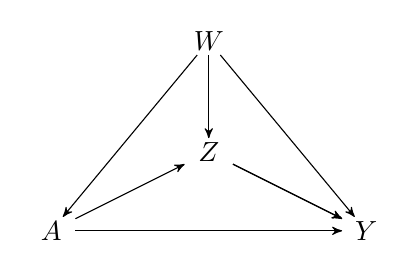
\begin{tikzpicture}
        \Vertex{0, 1.41}{W}
        \Vertex{0, 0}{Z}
        \Vertex{-2, -1}{A}
        \Vertex{2, -1}{Y}
        \Arrow{W}{A}{black}
        \Arrow{A}{Z}{black}
        \Arrow{Z}{Y}{black}
        \Arrow{Z}{Y}{black}
        \Arrow{W}{Y}{black}
        \Arrow{A}{Y}{black}
        \Arrow{W}{Z}{black}
      \end{tikzpicture}
    % \caption{Directed Acyclic Graph.}
    % \label{fig:dag}
    \end{figure}

\note{
}

\end{frame}

%%%%%%%%%%%%%%%%%%%%%%%%%%%%%%%%%%%%%%%%%%%%%%%%%%%%%%%%%%%%%%%%%%%%%%%%%%%%%%%%

\begin{frame}{Natural (in)direct effects}

Counterfactuals:
  \[Y(1) = f_Y(W, 1, Z(1), U_Y);\quad\quad Y(0) = f_Y(W, 0, Z(0),
    U_Y)\]
Average treatment effect:
  \begin{align*}
   \psi_{\text{ATE}} &= \E\{Y(1) - Y(0)\}\\
                 &=\underbrace{\E\{Y(1, Z(1)) -
                   Y(1, Z(0))\}}_{\text{natural indirect effect}} +
                   \underbrace{\E\{Y(1, Z(0)) -
                   Y(0, Z(0))\}}_{\text{natural direct effect}}
  \end{align*}
  \begin{block}{Problems}
    \begin{itemize}
      \item Focuses on binary exposures and static interventions
      \item Needs cross-world counterfactual independencies
      \item Requires identification of the exposure-mediator effect
      \item Requires positivity of exposure and mediator mechanisms
    \end{itemize}
  \end{block}

\note{
  \begin{itemize}
    \item ``Cross-world'' counterfactual independencies: independencies on
      counterfactual variables indexed by distinct hypothetical interventions.
    \item Consequently, these effects are not identifiable in a randomized
    trial (no valid randomization that performs the joint intervention); thus,
    scientific claims obtained from these models are not falsifiable through
    experimentation.
  \item Two routes around ``cross-world'': set identification (of bounds) and
    alternative effect definitions.
\end{itemize}
}

\end{frame}

%%%%%%%%%%%%%%%%%%%%%%%%%%%%%%%%%%%%%%%%%%%%%%%%%%%%%%%%%%%%%%%%%%%%%%%%%%%%%%%%

\begin{frame}{Stochastic interventions}
  \begin{definition}
    \textit{Stochastic interventions} yield a post-intervention exposure that
    is itself a random variable after conditioning on covariates $W$.
  \end{definition}

\vspace{2mm}

  We will study two types of stochastic interventions:
  \begin{itemize}
    \item Modified treatment policies $d(A,W)$.
    \item Exponential tilting.
  \end{itemize}

\note{
}

\end{frame}

%%%%%%%%%%%%%%%%%%%%%%%%%%%%%%%%%%%%%%%%%%%%%%%%%%%%%%%%%%%%%%%%%%%%%%%%%%%%%%%%

\begin{frame}{Modified treatment policies}
    \begin{itemize}
      \item Consider a hypothetical world where the treatment received is
        some function $d(A,W)$ of the treatment \textit{actually} received
        $A$ and covariates $W$.
    \end{itemize}
    \begin{example}[\cite{haneuse2013estimation}]
      \begin{itemize}
        \item What is the impact of operating time on outcomes for patients
          undergoing surgical resection for non-small-cell lung cancer.
        \item We can answer this using a hypothetical intervention
          $d(A,W) = A-\delta$ for user-supplied $\delta$.
        \item Denote the post-intervention exposure $A_\delta = d(A,W)$
        \item Non-parametric definition of effects with an interpretation
          that is familiar to users of OLS regression adjustment.
        \item Requires assuming piecewise smooth invertibility of
        $d(\cdot, w)$.
      \end{itemize}
    \end{example}

\note{
}

\end{frame}

%%%%%%%%%%%%%%%%%%%%%%%%%%%%%%%%%%%%%%%%%%%%%%%%%%%%%%%%%%%%%%%%%%%%%%%%%%%%%%%%

\begin{frame}{Exponential tilting}
  \begin{itemize}
  \item Consider an intervention that changes the exposure distribution
    conditional on covariates from $g(a\mid w)$ to
    $g_\delta(a\mid w)$, where
    \begin{equation*}
      g_\delta(a \mid w) \propto \exp(\delta a) g(a \mid w)
    \end{equation*}
  \item Denote by $A_\delta$ a draw from post-intervention distribution
    $g_\delta$.
  \end{itemize}
  \begin{example}[\cite{kennedy2017nonparametric}]
    \begin{itemize}
    \item \textit{Incremental propensity score interventions.} For binary $A$,
      \begin{equation*}
        g_\delta(1 \mid w) = \frac{\delta g(1 \mid w)}{\delta g(1 \mid w) + 1
          - g(1\mid w)},
      \end{equation*}

    \item Here, $\odds\{A_\delta= 1\mid W=w\} = \delta\odds\{A=1\mid W=w\}$.
    \end{itemize}
  \end{example}

\note{
}

\end{frame}

%%%%%%%%%%%%%%%%%%%%%%%%%%%%%%%%%%%%%%%%%%%%%%%%%%%%%%%%%%%%%%%%%%%%%%%%%%%%%%%%

\begin{frame}{Population intervention effect}
  \begin{itemize}
  \item For $A_\delta= d(A,W)$ (modified treatment policy), or $A_\delta$
   being a draw from $g_\delta(\cdot\mid W)$, define the population
   intervention effect (PIE) of $A$ on $Y$ as
    \begin{align*}
        \psi_{\text{PIE}}(\delta) &= \E\{Y(A_\delta) - Y\}\\
                     &=\underbrace{\E\{Y(A_{\delta}, Z(A_{\delta})) -
          Y(A_\delta, Z)\}}_{\text{indirect effect}} +
          \underbrace{\E\{Y(A_\delta, Z) -
          Y(A, Z)\}}_{\text{direct effect}}.
    \end{align*}
  \item Identification and estimation of $\E\{Y(A_{\delta}, Z(A_{\delta})\}$
    has been done \cite[e.g.,][]{diaz2012population,kennedy2017nonparametric}.
  \item \cite{diaz2020causal} focus on the decomposition term
    $\theta(\delta) = \E\{Y(A_{\delta}, Z)\}$
  \end{itemize}

\note{
}

\end{frame}

%%%%%%%%%%%%%%%%%%%%%%%%%%%%%%%%%%%%%%%%%%%%%%%%%%%%%%%%%%%%%%%%%%%%%%%%%%%%%%%%

\begin{frame}{Identification}
  \begin{itemize}
  \item \textit{Common support:}\newline $\supp\{g_\delta(\, \cdot \mid w)\}
     \subseteq \supp\{g(\, \cdot \mid w)\}$
  \item \textit{Conditional exchangeability:}
    $\E\{Y(a, z) \mid A, W, Z\}=\E\{Y(a, z) \mid W, Z\}$
  \end{itemize}
\begin{columns}[c]
  \column{0.5 \textwidth}
  \begin{figure}[!htb]
    \centering
    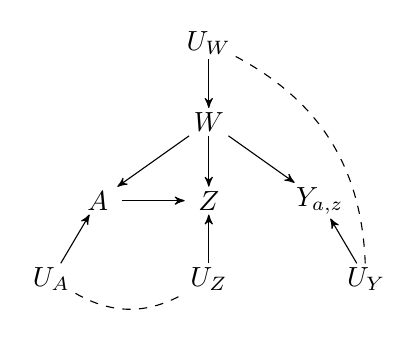
\begin{tikzpicture}
      \Vertex{0, 1}{U_W}
      \Vertex{0, 0}{W}
      \Vertex{0, -1}{Z}
      \Vertex{0, -2}{U_Z}
      \Vertex{-1.41, -1}{A}
      \Vertex{-2, -2}{U_A}
      \Vertex{1.41, -1}{Y_{a,z}}
      \Vertex{2, -2}{U_Y}
      \Arrow{W}{A}{black}
      \Arrow{U_A}{A}{black}
      \Arrow{U_Y}{Y_{a,z}}{black}
      \Arrow{U_W}{W}{black}
      \Arrow{U_Z}{Z}{black}
      \Arrow{A}{Z}{black}
      \Arrow{W}{Y_{a,z}}{black}
      \Arrow{W}{Z}{black}
      \EdgeR{U_Y}{U_W}{black}
      \EdgeR{U_A}{U_Z}{black}
    \end{tikzpicture}
    % \caption{Directed Acyclic Graph.}
    \label{fig:dag}
  \end{figure}
  \column{0.5 \textwidth}
  \begin{figure}[!htb]
    \centering
    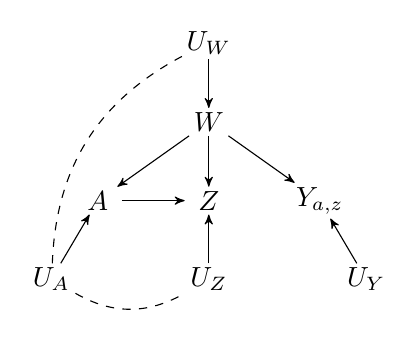
\begin{tikzpicture}
      \Vertex{0, 1}{U_W}
      \Vertex{0, 0}{W}
      \Vertex{0, -1}{Z}
      \Vertex{0, -2}{U_Z}
      \Vertex{-1.41, -1}{A}
      \Vertex{-2, -2}{U_A}
      \Vertex{1.41, -1}{Y_{a,z}}
      \Vertex{2, -2}{U_Y}
      \Arrow{W}{A}{black}
      \Arrow{U_A}{A}{black}
      \Arrow{U_Y}{Y_{a,z}}{black}
      \Arrow{U_W}{W}{black}
      \Arrow{U_Z}{Z}{black}
      \Arrow{A}{Z}{black}
      \Arrow{W}{Y_{a,z}}{black}
      \Arrow{W}{Z}{black}
      \EdgeL{U_A}{U_W}{black}
      \EdgeR{U_A}{U_Z}{black}
    \end{tikzpicture}
    % \caption{Directed Acyclic Graph.}
    \label{fig:dag}
  \end{figure}
\end{columns}

\note{
}

\end{frame}

%%%%%%%%%%%%%%%%%%%%%%%%%%%%%%%%%%%%%%%%%%%%%%%%%%%%%%%%%%%%%%%%%%%%%%%%%%%%%%%%

\begin{frame}{Identification}
  \begin{equation*}
    \theta(\delta) = \int m(a, z,
    w)g_\delta(a\mid w)p(z,w)\dd\nu(a,z,w),
  \end{equation*}
where $m(a, z, w) = \E(Y\mid A=a, Z=z, W=w)$.
  \begin{block}{Compared to the natural (in)direct effects:}
    \begin{itemize}
    \item No cross-world independence assumptions.
    \item No need to identify exposure-mediator effect.
    \item Positivity guaranteed by definition.
    \item Allows nonparametric effects for continuous exposures.
    \end{itemize}
  \end{block}

\note{
}

\end{frame}

%%%%%%%%%%%%%%%%%%%%%%%%%%%%%%%%%%%%%%%%%%%%%%%%%%%%%%%%%%%%%%%%%%%%%%%%%%%%%%%%

\begin{frame}{G-computation and IPW estimation}
  \begin{eqnarray*}
    \theta(\delta) &=& \E\left\{\int m(a, Z, W)
                       g_\delta(a \mid W)\dd\nu(a) \right\}\label{eq:gcomp}\\
                     % &=&E\left\{\frac{g_\delta(a\mid w)p(z\mid
                     %   w)}{g(a\mid w)p(z\mid a, w)}\, Y\right\},\notag\\
                   &=& \E \left\{\frac{g_\delta(A \mid W)}
                       {e(A \mid Z, W)}\, Y \right\},
  \end{eqnarray*}
  where $e$ is the pdf of $A\mid Z,W$:
  \[e(a \mid z, w) = \frac{g(a\mid w) p(z\mid a, w)}{p(z\mid w)}.\]
  \begin{itemize}
  \item The above formulas may be used to construct the classical G-computation
    and IPW estimators.
  \item If the nuisance parameters estimators are data-adaptive, G-computation
    and IPW generally fail to be $n^{1/2}$-consistent.
  \end{itemize}

\note{
}

\end{frame}

%%%%%%%%%%%%%%%%%%%%%%%%%%%%%%%%%%%%%%%%%%%%%%%%%%%%%%%%%%%%%%%%%%%%%%%%%%%%%%%%

\begin{frame}{Efficient one-step estimator}
  \begin{itemize}
  \item \textit{Main idea:} Find $D_P(o)$ such that:
    \[\theta_{\hat P}(\delta) - \theta_P(\delta) = -\E\{ D_{\hat
        P}(O)\} + O\big(||\hat P - P||^2\big)\]
  \item De-bias $\theta_{\hat P}(\delta)$ by computing
    \[\tilde \theta(\delta) = \theta_{\hat P}(\delta) +
      \frac{1}{n}\sum_{i=1}^n D_{\hat P}(O_i)\]
  \item In the nonparametric model there is only one such $D_P$; it
    is referred to as \textit{canonical gradient} or \textit{efficient
      influence function}.
  \end{itemize}

\note{
}

\end{frame}

%%%%%%%%%%%%%%%%%%%%%%%%%%%%%%%%%%%%%%%%%%%%%%%%%%%%%%%%%%%%%%%%%%%%%%%%%%%%%%%%

\begin{frame}[c]{Efficient Influence Function for $\theta(\delta)$}

\begin{center}
\begin{itemize}
\itemsep2pt
\item For simplicity, let $A \in \{0, 1\}$ and consider incremental propensity
  score interventions \citep{kennedy2017nonparametric}, EIF given as
  \vspace{-0.5em}
  \begin{align*}
    D^{Z, W}_{\eta, \delta}(o) &= \int m(z, a, w) g_{\delta}(a \mid w)
      d\kappa(a)\\
    D^Y_{\eta, \delta}(o) &= \mathbf{\textcolor{blue}{\frac{g_{\delta}
    (a \mid w)} {e(a \mid z, w)}}} \{y - m(z,a,w) \},\\
    D^A_{\eta,\delta}(o) &= \frac{\mathbf{\textcolor{red}{\delta\phi(w)}}\{a -
      g(1 \mid w)\}}{\mathbf{\textcolor{red}{\{\delta g(1 \mid w) +
      g(0 \mid w)\}^2}}},
  \end{align*}
  where $\phi(w) = \mathbb{E}\left\{m(1, Z, W) - m(0, Z, W) \mid W = w
  \right\}$.
\item For an unabridged treatment, see~\cite{diaz2020causal}.
\item Original work does not construct a TML estimator.
\end{itemize}
\end{center}

\note{
}

\end{frame}


%%%%%%%%%%%%%%%%%%%%%%%%%%%%%%%%%%%%%%%%%%%%%%%%%%%%%%%%%%%%%%%%%%%%%%%%%%%%%%%%

\begin{frame}{Weak convergence for exponential tilting}
  \begin{itemize}
    \item $D_P$ does not depend on all of $P$, just on $\eta=(m,g,e,\phi)$.
    \item Construct cross-validated estimates of $m$, $g$, $e$, $\phi$ ---
      i.e., for computing $\hat m(O_i)$, use training data not containing $O_i$.
  \item Assume convergence of certain second-order terms --- e.g.,
    $\lVert \hat{m} - m\rVert \lVert\hat{g} - g\rVert = o_P(n^{-1/2})$.
  \item Then,
        $\sqrt{n}\{\tilde \theta(\delta) - \theta(\delta)\} \rightsquigarrow
          N(0;\var\{D_{\eta} (O)\})$.
   \item This result can be made uniform in intervals $[\delta_l,\delta_u]$
  \item Uniform result can be used to test the hypothesis of no
    direct effect \citep{kennedy2017nonparametric}:
    $H_0 : \sup_{\delta \in \Delta} \theta(\delta) = \E(Y)$.
  \end{itemize}

\note{
}

\end{frame}

%%%%%%%%%%%%%%%%%%%%%%%%%%%%%%%%%%%%%%%%%%%%%%%%%%%%%%%%%%%%%%%%%%%%%%%%%%%%%%%%

\begin{frame}{Multiple robustness}
  \begin{itemize}
  \item \textit{Modified treatment policies:} Assume piecewise smooth
    invertibility of $d(\cdot, w)$, and define $r(z\mid w) = p(z\mid w)$.
    Consistency requires:
    \begin{enumerate}
      \item $g_1=g$ and either $e_1=e$ or $m_1=m$, or
      \item $m_1=m$ and either $g_1=g$ or $r_1=r$.
    \end{enumerate}
    Intuition: use change of variable formula to get
    \[\theta(\delta) = \E\left\{\int m(d(A,W),z,W)r(z \mid,
        W)\dd\nu(z)\right\}.\]
  \item \textit{Exponential tilt:} consistency requires that $g_1 = g$ and
     either $e_1 = e$ or $m_1 = m$.
  \end{itemize}

\note{
}

\end{frame}

%%%%%%%%%%%%%%%%%%%%%%%%%%%%%%%%%%%%%%%%%%%%%%%%%%%%%%%%%%%%%%%%%%%%%%%%%%%%%%%%

\begin{frame}[c]{TML Estimator for $\theta(\delta)$}

\begin{center}
\begin{itemize}
\itemsep2pt
\item We can construct a TML estimator by using the EIF to update initial
  estimates of nuisance parameters:
    \begin{equation*}
      \hat{\theta}_{\text{TMLE}}(\delta) = \int \frac{1}{n} \sum_{i=1}^n
      \hat{m}^{\star}_{j(i)}(Z, a, W)
      \hat{g}_{\delta, j(i)}^{\star}(a \mid W) d\kappa(a).
    \end{equation*}
  \item TMLE constructs a substitution estimator, respecting bounds.
  \item Avoid entropy conditions by cross-validation \citep{zheng2011cross,
    chernozhukov2016double}, so let $j(i)$ be the index of the validation set
    containing observation $i$.
  \item Use universal least favorable submodels \citep{vdl2016one} for the
    targeting step.
\end{itemize}
\end{center}

\note{
}

\end{frame}

%%%%%%%%%%%%%%%%%%%%%%%%%%%%%%%%%%%%%%%%%%%%%%%%%%%%%%%%%%%%%%%%%%%%%%%%%%%%%%%%

\begin{frame}[c]{Targeting Step of TMLE for $\theta(\delta)$}

\begin{center}
\begin{itemize}
  \itemsep8pt
  \item $\hat{g}_{\delta}^{\star}(a \mid w)$ generated via \textit{targeting}
    fluctuation that tilts initial estimates towards solutions of the score
    $\frac{1}{n}\sum_{i=1}^n D^A(O_i) = 0$:
    $\text{logit}(\hat{g}_{\delta,k\xi}) =
    \text{logit}(\hat{g}_{\delta,(k-1)\xi}) + \xi_{\Delta g}^{\text{lfm}}
    \mathbf{\textcolor{red}{H^A_{(k-1)\xi}}}$
    \begin{itemize}
      \itemsep4pt
      \item Take $\hat{g}_{\delta,k\xi}$ in final step as
        $\hat{g}_{\delta}^{\star}(a \mid w)$.
      \item Use the term before the residual $a - g(1 \mid w)$ in $D^A$ as the
        covariate in this regression (treating initial estimate as offset).
    \end{itemize}
  \item Similarly for $\hat{m}^{\star}(z,a,w)$ but to solve
    $\frac{1}{n}\sum_{i=1}^n D^Y(O_i) = 0$:
    $\text{logit}(\hat{m}_{k\xi}) = \text{logit}(\hat{m}_{(k-1)\xi}) +
    \xi_{\Delta m}^{\text{lfm}}
    \mathbf{\textcolor{blue}{H^Y_{(k-1)\xi}}}$.
    \begin{itemize}
      \itemsep4pt
      \item Take $\hat{m}_{k\xi}$ in final step as
        $\hat{m}^{\star}_{j(i)}(Z, a, W)$.
      \item Use the term before the residual $y - m(z,a,w)$ in $D^Y$ as the
        covariate in this regression (treating initial estimate as offset).
  \end{itemize}
\end{itemize}
\end{center}

\note{
\begin{itemize}
  %\item Could also do less aggressive targeting as per~\cite{pmlr-v97-bibaut19a}.
  \item Stops when appropriate component of EIF is nearly solved, i.e.,
    $\frac{1}{n}\sum_{i=1}^n D^{\{Y, A\}}(O_i) < \frac{1}{n}$ or
    $\frac{\sigma^2(D)}{\log n}$.
\end{itemize}
}

\end{frame}

%%%%%%%%%%%%%%%%%%%%%%%%%%%%%%%%%%%%%%%%%%%%%%%%%%%%%%%%%%%%%%%%%%%%%%%%%%%%%%%%

\begin{frame}[c]{Software implementation}

\begin{center}
\begin{itemize}
  \itemsep2pt
  \item The \underline{\texttt{medshift} \texttt{R} package}
    \citep{hejazi2020medshift} implements TML estimator with state-of-the-art
    machine learning.
    \begin{itemize}
      \item Access all estimators via the eponymous \texttt{medshift()}
        function.
      \item Uses the \texttt{sl3} \texttt{R} package for ensemble machine
        learning.
      \item Relies on the \texttt{tmle3} framework for the TMLE implementation.
      \item Cross-fitting implementation via the \texttt{origami} \texttt{R}
        package.
    \end{itemize}
  \item \texttt{sl3}, \texttt{tmle3}, and \texttt{origami} are the 3 core
    engines of the \textbf{\texttt{tlverse}} software ecosystem
    (\url{https://tlverse.org}).
    \begin{itemize}
      \item Our handbook: \url{https://tlverse.org/tlverse-handbook}
    \end{itemize}
\end{itemize}
\includegraphics[origin=c,scale=0.3]{tlverse}
\end{center}

\note{
}

\end{frame}


%%%%%%%%%%%%%%%%%%%%%%%%%%%%%%%%%%%%%%%%%%%%%%%%%%%%%%%%%%%%%%%%%%%%%%%%%%%%%%%%

\begin{frame}{Numerical studies}
  \begin{figure}[H]
    \hspace*{-1.5cm}
    \centering
    \includegraphics[scale=0.3]{plot_jrssb}
    % \caption{Statistics for the three key estimators (and variations
    %   thereof) of the direct effect under an IPS intervention
    %   $\delta = 0.5$, across $1000$ Monte Carlo simulations for each of
    %   seven sample sizes.}
    % \label{fig:all_metric_comparison}
  \end{figure}

\note{
}

\end{frame}

%%%%%%%%%%%%%%%%%%%%%%%%%%%%%%%%%%%%%%%%%%%%%%%%%%%%%%%%%%%%%%%%%%%%%%%%%%%%%%%%

\begin{frame}{Some notes and next steps}
  \begin{itemize}
  \item Nonparametric efficient estimation of effects using
    data-adaptive regression and cross-validation
    \begin{itemize}
      \item Avoid reliance on misspecified parametric models.
      \item Cross-validation helps keep the function classes unrestricted.
    \end{itemize}
  \item Working on adaptations to mediator-outcome confounders
    affected by treatment.
  \item \texttt{R} package: \url{https://github.com/nhejazi/medshift}
  \item Integrated in the \texttt{tlverse} targeted learning ecosystem
  \item Paper (JRSS-B): \url{https://doi.org/10.1111/rssb.12362}
  \item arXiv pre-print: \url{https://arxiv.org/abs/1901.02776}
  \item We would love to hear your input:
    \begin{itemize}
    \item[-] ild2005@med.cornell.edu
    \item[-] nhejazi@berkeley.edu
    \end{itemize}
  \end{itemize}

\note{
}

\end{frame}

%%%%%%%%%%%%%%%%%%%%%%%%%%%%%%%%%%%%%%%%%%%%%%%%%%%%%%%%%%%%%%%%%%%%%%%%%%%%%%%%

% don't want dimming with references
\setbeamercovered{}
\beamerdefaultoverlayspecification{}

\begin{frame}[c,allowframebreaks]{}

\scriptsize
\bibliographystyle{apalike}
\bibliography{references}

\end{frame}

%%%%%%%%%%%%%%%%%%%%%%%%%%%%%%%%%%%%%%%%%%%%%%%%%%%%%%%%%%%%%%%%%%%%%%%%%%%%%%%%

\begin{frame}[c]{Thank you.}

\large
Slides: \href{http://bit.ly/2020\_berkeley\_medshift}{bit.ly/2020\_berkeley\_medshift}
  \quad \includegraphics[height=4mm]{cc-zero.png}

\vspace{2mm}
\includegraphics[scale=0.14]{homepage.png} \url{https://nimahejazi.org}

\vspace{2mm}
\includegraphics[scale=0.11]{github-icon.png}
  \url{https://github.com/nhejazi}

\vspace{2mm}
\includegraphics[scale=0.14]{twitter-icon.png}
  \url{https://twitter.com/nshejazi}

\end{frame}

%%%%%%%%%%%%%%%%%%%%%%%%%%%%%%%%%%%%%%%%%%%%%%%%%%%%%%%%%%%%%%%%%%%%%%%%%%%%%%%%

\appendix
\begin{frame}[standout]
  Appendix
\end{frame}

\begin{frame}[c]{\cite{haneuse2013estimation}}

\begin{center}
\begin{itemize}
  \itemsep10pt
  \item \textit{Proposal:} Characterization of stochastic interventions as
    \textit{modified treatment policies} (MTPs).
  \item Assumption of \textit{piecewise smooth invertibility} allows for the
    intervention distribution of any MTP to be recovered:
    \begin{equation*}
      g_{0, \delta}(a \mid w) = \sum_{j = 1}^{J(w)} I_{\delta, j} \{h_j(a, w),
      w\} g_0\{h_j(a, w) \mid w\} h^{'}_j(a,w)
    \end{equation*}
  \item Such intervention policies account for the natural value of the
    intervention $A$ directly yet are interpretable as the imposition of an
    altered intervention mechanism.
  \item Identification conditions for assessing the parameter of interest under
    such interventions appear technically complex (at first).
\end{itemize}
\end{center}

\note{
  \begin{itemize}
    \item Shifts of the form $d(A,W)$ are considerably more interesting since
      these are realistic intervention policies.
    \item Example: consider an individual with an extremely high immune response
      but whose baseline covariates $W$ suggest we shift the response still
      higher. Such a shift may not be biologically plausible (impossible, even)
      but we cannot account for this if the shift is only a function of $W$.
    \item The authors build IPW, outcome regression, and non-iterative doubly
      robust estimators, as well as an approach based on MSMs.
    \item Piecewise smooth invertibility: This assumption ensures that we can
      use the change of variable formula when computing integrals over $A$ and
      it is useful to study the estimators that we propose in this paper.
  \end{itemize}
}

\end{frame}

\end{document}
